% Options for packages loaded elsewhere
\PassOptionsToPackage{unicode}{hyperref}
\PassOptionsToPackage{hyphens}{url}
%
\documentclass[
]{article}
\usepackage{amsmath,amssymb}
\usepackage{iftex}
\ifPDFTeX
  \usepackage[T1]{fontenc}
  \usepackage[utf8]{inputenc}
  \usepackage{textcomp} % provide euro and other symbols
\else % if luatex or xetex
  \usepackage{unicode-math} % this also loads fontspec
  \defaultfontfeatures{Scale=MatchLowercase}
  \defaultfontfeatures[\rmfamily]{Ligatures=TeX,Scale=1}
\fi
\usepackage{lmodern}
\ifPDFTeX\else
  % xetex/luatex font selection
\fi
% Use upquote if available, for straight quotes in verbatim environments
\IfFileExists{upquote.sty}{\usepackage{upquote}}{}
\IfFileExists{microtype.sty}{% use microtype if available
  \usepackage[]{microtype}
  \UseMicrotypeSet[protrusion]{basicmath} % disable protrusion for tt fonts
}{}
\makeatletter
\@ifundefined{KOMAClassName}{% if non-KOMA class
  \IfFileExists{parskip.sty}{%
    \usepackage{parskip}
  }{% else
    \setlength{\parindent}{0pt}
    \setlength{\parskip}{6pt plus 2pt minus 1pt}}
}{% if KOMA class
  \KOMAoptions{parskip=half}}
\makeatother
\usepackage{xcolor}
\usepackage[margin=1in]{geometry}
\usepackage{longtable,booktabs,array}
\usepackage{calc} % for calculating minipage widths
% Correct order of tables after \paragraph or \subparagraph
\usepackage{etoolbox}
\makeatletter
\patchcmd\longtable{\par}{\if@noskipsec\mbox{}\fi\par}{}{}
\makeatother
% Allow footnotes in longtable head/foot
\IfFileExists{footnotehyper.sty}{\usepackage{footnotehyper}}{\usepackage{footnote}}
\makesavenoteenv{longtable}
\usepackage{graphicx}
\makeatletter
\def\maxwidth{\ifdim\Gin@nat@width>\linewidth\linewidth\else\Gin@nat@width\fi}
\def\maxheight{\ifdim\Gin@nat@height>\textheight\textheight\else\Gin@nat@height\fi}
\makeatother
% Scale images if necessary, so that they will not overflow the page
% margins by default, and it is still possible to overwrite the defaults
% using explicit options in \includegraphics[width, height, ...]{}
\setkeys{Gin}{width=\maxwidth,height=\maxheight,keepaspectratio}
% Set default figure placement to htbp
\makeatletter
\def\fps@figure{htbp}
\makeatother
\setlength{\emergencystretch}{3em} % prevent overfull lines
\providecommand{\tightlist}{%
  \setlength{\itemsep}{0pt}\setlength{\parskip}{0pt}}
\setcounter{secnumdepth}{5}
% definitions for citeproc citations
\NewDocumentCommand\citeproctext{}{}
\NewDocumentCommand\citeproc{mm}{%
  \begingroup\def\citeproctext{#2}\cite{#1}\endgroup}
\makeatletter
 % allow citations to break across lines
 \let\@cite@ofmt\@firstofone
 % avoid brackets around text for \cite:
 \def\@biblabel#1{}
 \def\@cite#1#2{{#1\if@tempswa , #2\fi}}
\makeatother
\newlength{\cslhangindent}
\setlength{\cslhangindent}{1.5em}
\newlength{\csllabelwidth}
\setlength{\csllabelwidth}{3em}
\newenvironment{CSLReferences}[2] % #1 hanging-indent, #2 entry-spacing
 {\begin{list}{}{%
  \setlength{\itemindent}{0pt}
  \setlength{\leftmargin}{0pt}
  \setlength{\parsep}{0pt}
  % turn on hanging indent if param 1 is 1
  \ifodd #1
   \setlength{\leftmargin}{\cslhangindent}
   \setlength{\itemindent}{-1\cslhangindent}
  \fi
  % set entry spacing
  \setlength{\itemsep}{#2\baselineskip}}}
 {\end{list}}
\usepackage{calc}
\newcommand{\CSLBlock}[1]{\hfill\break\parbox[t]{\linewidth}{\strut\ignorespaces#1\strut}}
\newcommand{\CSLLeftMargin}[1]{\parbox[t]{\csllabelwidth}{\strut#1\strut}}
\newcommand{\CSLRightInline}[1]{\parbox[t]{\linewidth - \csllabelwidth}{\strut#1\strut}}
\newcommand{\CSLIndent}[1]{\hspace{\cslhangindent}#1}
\usepackage{pdflscape}
\usepackage{graphicx}
\usepackage{booktabs}
\usepackage{longtable}
\usepackage{array}
\usepackage{multirow}
\usepackage{wrapfig}
\usepackage{float}
\usepackage{colortbl}
\usepackage{pdflscape}
\usepackage{tabu}
\usepackage{threeparttable}
\usepackage{threeparttablex}
\usepackage[normalem]{ulem}
\usepackage{makecell}
\usepackage{xcolor}
\ifLuaTeX
  \usepackage{selnolig}  % disable illegal ligatures
\fi
\usepackage{bookmark}
\IfFileExists{xurl.sty}{\usepackage{xurl}}{} % add URL line breaks if available
\urlstyle{same}
\hypersetup{
  pdftitle={The Price of Dark Traits: Strategic Exploitation and Its Limitations in Repeated Trust Games},
  pdfauthor={Ismail Guennouni1,2,3,4*, Christoph Korn4, Georgia Koppe1,2,3},
  hidelinks,
  pdfcreator={LaTeX via pandoc}}

\title{The Price of Dark Traits: Strategic Exploitation and Its Limitations in Repeated Trust Games}
\author{Ismail Guennouni\textsuperscript{1,2,3,4}*, Christoph Korn\textsuperscript{4}, Georgia Koppe\textsuperscript{1,2,3}}
\date{2025-03-28}

\begin{document}
\maketitle
\begin{abstract}
Trust and cooperation are fundamental to human social interaction, with personality traits significantly influencing economic decision-making. This study examines how the Dark Factor of Personality (D-factor) affects behavior in repeated trust games. After pre-screening 1,243 participants, we selected groups with high (N=91) and low (N=92) D-factor scores. Participants played two 25-round trust games as trustees against different Hidden Markov Model investors: one ``human-like'' with stable response patterns and one ``responsive'' that changed trust states more readily based on participants' return behavior. High D-factor participants consistently returned lower proportions, particularly in later rounds, and strategically decreased reciprocity over time when receiving high investments from predictable opponents. Despite exploitative behavior, high D-factor participants did not achieve higher total payoffs, as the adaptive opponents reduced investments in response to lower returns. These findings demonstrate how dark personality traits manifest in dynamic economic exchanges and highlight the sophisticated yet ultimately self-limiting nature of exploitation in responsive social environments.
\end{abstract}

\small

\textsuperscript{1} \emph{Department of Psychiatry and Psychotherapy, Central Institute of
Mental Health, Medical Faculty Mannheim, Heidelberg University,
Mannheim, Germany}

\textsuperscript{2} \emph{Interdisciplinary Center for Scientific Computing, Faculty of
Mathematics and Computer Science, Heidelberg University, Heidelberg,
Germany}

\textsuperscript{3} \emph{Hector Institute for AI in Psychiatry, Central Institute of Mental
Health, Medical Faculty Mannheim, Heidelberg University, Mannheim
Germany}

\textsuperscript{4} \emph{Department of General Psychiatry, Section Social Neuroscience,
Heidelberg University, Germany}

\textsuperscript{*} \emph{Corresponding author. Address: Central Institute of Mental Health,
J5, Mannheim, Germany. Email:
\href{mailto:ismail.guennouni@iwr.uni-heidelberg.de}{ismail.guennouni@zi-mannheim.de}}

\pagebreak

\section{Introduction}\label{introduction}

Trust and cooperation are fundamental to human social interaction and economic exchange (Berg, Dickhaut, and McCabe 1995). The trust game, particularly in its repeated form, has emerged as a powerful tool for investigating the dynamics of trust and reciprocity in controlled settings (Camerer 2003). While numerous studies have explored various personality traits as predictors of behavior in trust games, recent developments in personality psychology offer new avenues for understanding the underlying factors that influence trustworthiness.

The Dark Factor of Personality (D-factor), proposed by Moshagen, Hilbig, and Zettler (2018), represents a unified construct encompassing various malevolent personality traits. Defined as the general tendency to maximize one's utility at the expense of others, accompanied by beliefs that serve as justifications, the D-factor offers a comprehensive framework for understanding antisocial tendencies. This construct incorporates elements of Machiavellianism, Narcissism, and Psychopathy - traits previously linked to reduced trustworthiness in economic games (Ibáñez et al. 2016; Gunnthorsdottir, McCabe, and Smith 2002).

Research has consistently demonstrated negative correlations between dark personality traits and cooperative behavior in various economic games. A meta-analysis by Zhao and Smillie (2015) found that dark triad traits negatively predict cooperation across different economic paradigms. Similarly, Thielmann and Hilbig (2019) observed that dark personality traits predict dishonest behavior in economic interactions. These findings suggest that the D-factor, as a unifying construct, may serve as a potent predictor of untrustworthy behavior in trust games.

While the D-factor has shown associations with selfish behavior in dictator games (Moshagen, Hilbig, and Zettler 2020) and lower levels of honesty-humility (Zettler, Moshagen, and Hilbig 2021), its specific impact on trustworthiness in repeated trust games remains unexplored. This gap is particularly notable given the unique features of the repeated trust game, which allows for the development of reputation and the potential for strategic behavior over multiple interactions (Bohnet and Huck 2004).
The repeated nature of the game introduces complexity not present in one-shot interactions. Individuals with high D-factor scores (High-D) may exhibit different patterns of behavior over repeated rounds compared to low D-factor scores individuals (Low-D), such as potentially engaging in strategic trust-building before exploitation. This dynamic aligns with the Machiavellian aspect of the D-factor, which involves a strategic, long-term orientation to personal gain (Jones and Paulhus 2009).

A notable exception is the study by Gong et al. (2019), which examined the relationship between psychopathic traits and behavior in a modified trust game. However, their design involved multiple different partners rather than repeated interactions with the same opponent. Similarly, Rosenberger, Tsivilis, and Müller (2019) examined fairness norm violations in violent offenders during a repeated trust game, finding that antisocial traits (Factor 2 of psychopathy) rather than interpersonal/affective traits (Factor 1) were associated with reduced reciprocity. However, this study focused on clinical psychopathy in offenders rather than the D-factor in the general population.

The present study addresses several important gaps in our understanding of how dark personality traits influence economic behavior. First, by using a repeated trust game paradigm with 25 rounds, we can examine whether High-D individuals demonstrate strategic patterns that evolve over time, such as initial trust-building followed by exploitation. Second, by manipulating opponent predictability through the use of different Hidden Markov Model (HMM) agents---one ``human-like'' and one more ``responsive''--- we can assess whether the behavioral manifestation of dark personality traits varies based on environmental stability. This approach allows us to test whether High-D individuals demonstrate sophisticated social intelligence by adapting their strategies to different counterparts.
The use of HMM agents as opponents provides significant methodological advantages for studying dark personality traits. These computational models, trained on real human behavior data, allow us to create standardized yet responsive interaction partners whose strategies can be precisely characterized and manipulated. This approach combines ecological validity (as the agents mimic actual human behavior) with experimental control, allowing us to isolate the effects of personality while maintaining the dynamic nature of trust interactions.

Understanding the D-factor's influence on trustworthiness has significant implications, bridging personality psychology and behavioral economics while potentially informing interventions to promote cooperation among those with High-D scores. The present study aims to investigate the predictive power of the Dark Factor of Personality on trustworthiness in the repeated trust game. We hypothesize that individuals scoring higher on the D-factor will exhibit less trustworthy behavior as trustees, particularly in later rounds of the game. Additionally, we expect High-D individuals to show greater strategic adaptation to opponent type, with more pronounced exploitation of predictable opponents compared to responsive ones. Finally, we explore whether these behavioral patterns are accompanied by systematic differences in perception of opponents, with High-D individuals potentially showing more negative evaluations regardless of opponent behavior.

\section{Methods}\label{methods}

\subsection{Participants}\label{participants}

To have participants with large differences in the D factor of personality, a total of 1243
participants were pre-screened on the Prolific Academic platform
(prolific.co) using the 16 item Dark Factor of Personality Questionnaire (D16) to
finally select two similarly sized groups: One with high D factor scores (90th percentile or higher, D score
\textgreater{} 42, N=91) and the other with low D factor scores (10th percentile, score \textless{} 22, N=92)
totaling 183 participants (44\% female). These were then invited through
prolific to take part in the main experiment.

To determine the appropriate sample size, we conducted an a priori power analysis using Monte Carlo simulations with the \emph{simr} package in R. The analysis specifically targeted the three-way interaction between d-score, opponent type (stable vs.~responsive), and investment level. Parameters for the simulation were based on previous studies, with an expected effect size of \(-0.1\) (correlation between d-score and returns), alpha level of \(0.05\), and desired power of \(0.90\). Starting with 50 participants, we iteratively generated synthetic data for a task with \(25\) rounds per condition and fitted linear mixed-effects models with random intercepts for participants. The simulations incorporated realistic parameter estimates and fixed effects derived from previous research using the same paradigm. This analysis indicated that a sample of 180 participants would provide at least \(90\%\) power to detect the hypothesized three-way interaction.

The mean age of participants was \(33.1\) years, with an \(9.7\)-year standard deviation. The majority of participants identified ethnically as White (\(57\)\%). The online cohort registered \(38\) unique countries of birth with the most frequent being South Africa (\(24\)\%), the U.K. (\(20\)\%) followed by Poland (\(5\)\%) and Greece (\(4\)\%). Participants were paid a fixed fee of £4 plus a bonus payment dependent on their performance that averaged £\(0.5\). We collected data over multiple sessions between October and November 2024.

\subsection{Design and Procedure}\label{design-and-procedure}

The experiment employed a 2 (HMM Type: Human-like or Responsive) × 2 (D-Factor: High or Low) mixed design, with repeated measures on the HMM Type factor. Participants were pre-screened using the 16-item Dark Personality Factor Questionnaire, with individuals classified as either High D or Low D. Participants completed two phases of a Repeated Trust Game (RTG), playing 25 rounds in each phase against different Hidden Markov Model (HMM) investors: a ``Human-like'' HMM and a more ``Responsive'' HMM, with the order counterbalanced across participants. After each RTG phase, participants completed investor evaluations. The experiment concluded with a Turing test to assess perceived humanness of the AI partners, open-ended questions about the interaction, and a final debrief. The experimental interface was designed and implemented online using Empirica v1 (Almaatouq et al. 2021), with an estimated completion time of 30 minutes per participant. The study received approval from the University of Heidelberg's Medical Faculty ethics commission (ID:S-708/2023) and the experiment was performed in accordance with the ethics board guidelines and regulations. All participants provided informed consent prior to their participation.

\begin{landscape}
\begin{figure}[htbp]
\centering
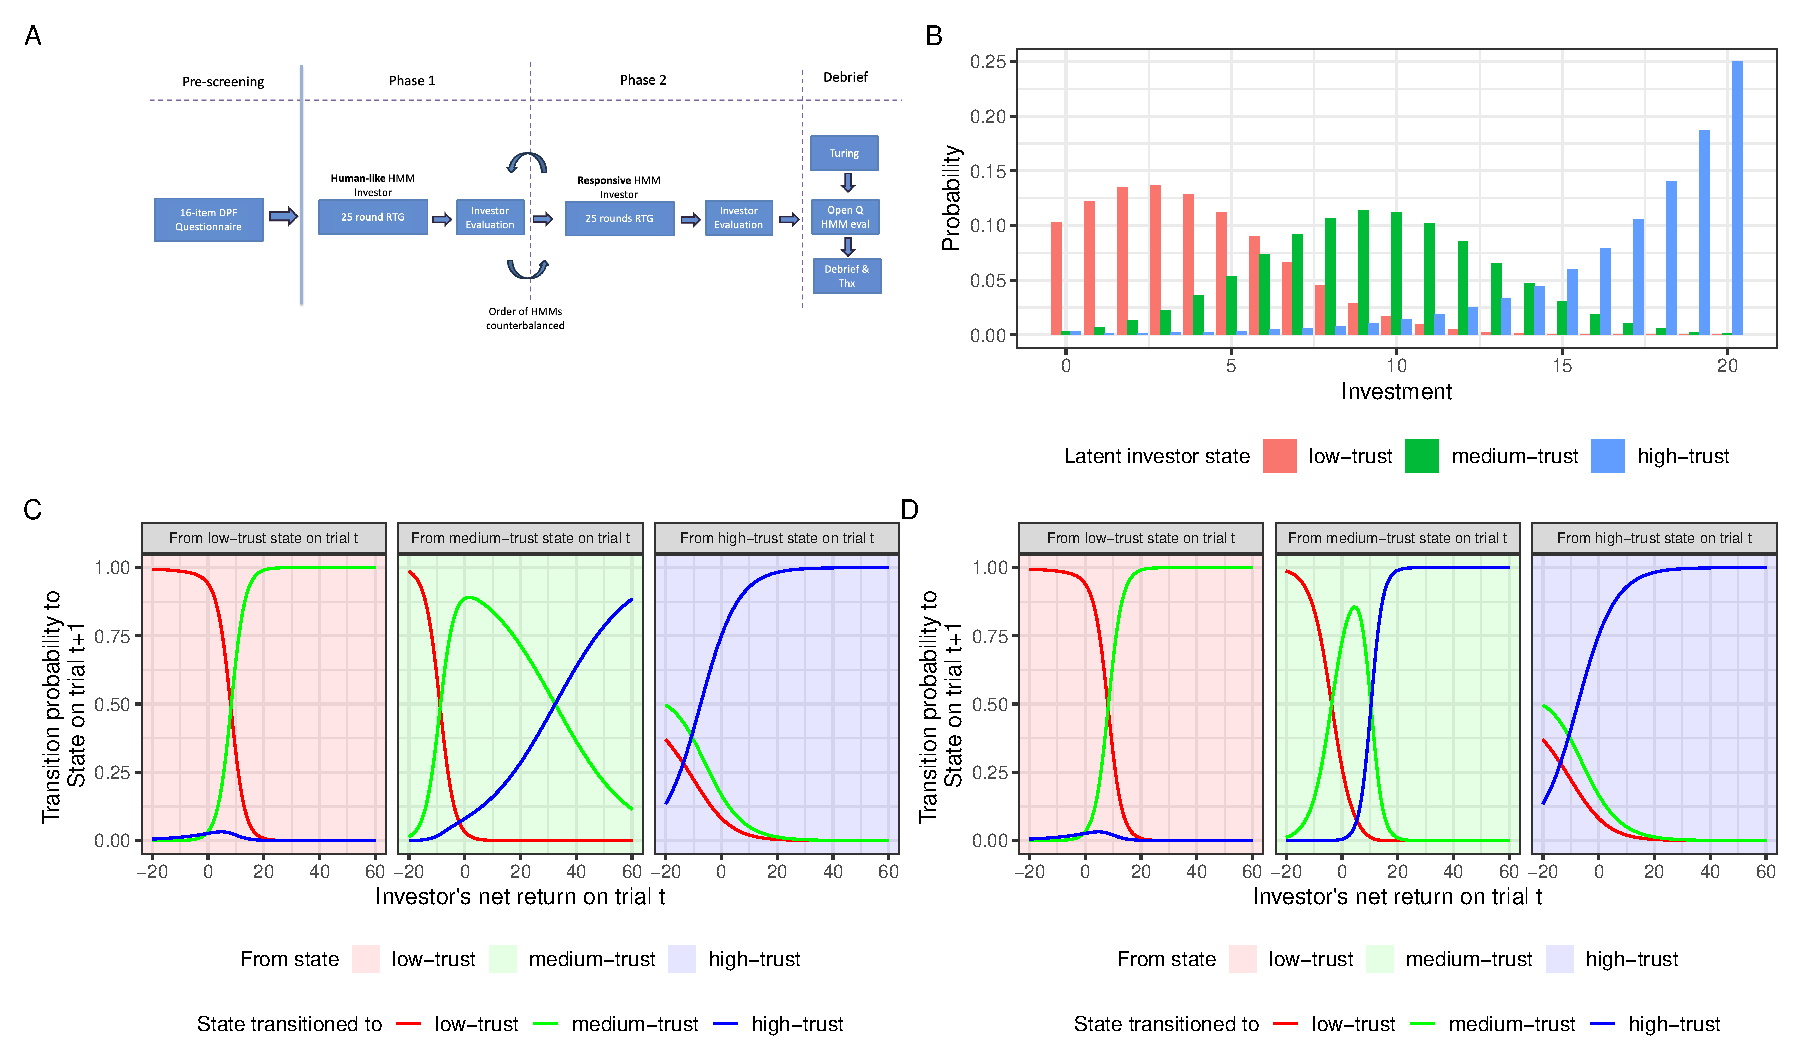
\includegraphics[width=\linewidth]{plots/figure1.pdf}
\caption{\small{Panel A: A timeline of the experiment. The RTG is played in dyads, with participants always assigned the role of the trustee and the HMM agent that of the investor. The investor is endowed with 20 units at the start of each round. They need to decide how much of that endowment they want to invest with the trustee. The investment is then multiplied by a factor of 3 and sent to the trustee who needs to decide how much of the multiplied investment they want to send back to the investor. The difference between phases is the type of agents participants are facing. Panels B - C: We construct the artificial investor agent by fitting a three-state hidden Markov model to data of human investors engaged in the 10 round RTG. From the fitted HMM, we get the distribution of investments by the human-like agent, conditional on its latent state as shown in Panel B. The fitted HMM also yields the transition probability of the agent to a state on trial t+1 as a function of the net return (difference between the investment sent and the amount received in return) on trial t as shown in Panel C. Each plot in Panel C represents a different starting latent state on trial t, and each line represents the probability of transitioning to a particular state in trial t+1. Panel D shows the transition probabilities of the responsive HMM agent. Unlike the human-like HMM, the responsive HMM is much more likely to transition out of the mid-trust state. Transitions in the medium and high trust states were identical for both agents.}}
\label{fig:combinedPlots}
\end{figure}
\end{landscape}

\subsection{Tasks and Measures}\label{tasks-and-measures}

\subsubsection{Repeated Trust Game and HMM Investor}\label{repeated-trust-game-and-hmm-investor}

Participants played a 25-round RTG (Berg, Dickhaut, and McCabe 1995) in the trustee
role against a computer-programmed investor. On each round, the investor
is endowed with 20 units and decides how much of that endowment to
invest. This investment is tripled and the trustee then decides how to
split this tripled amount between themselves and the investor. If the trustee
returns more than one third of the amount, the investor makes a gain.
Each player was represented with an icon with the participant always on
the left of the screen and the co-player on the right. The participants
were able to choose the icon that represents them at the start of the
experiment. The icon representing the co-player changed at the start of
each new game, to simulate a new interaction partner. Participants were
not told they were facing computerised co-players. We chose to simulate
the behavior of a human interaction partner through allowing for a delay
while pairing with new opponents as the start of each game as well as
programming the agents to respond during each round after a varying time
lapse (randomly chosen between 5 and 10 seconds).

The computerised investor consisted of a hidden Markov model (HMM)
trained on an independent existing behavioral RTG data set of human
investors. This data-driven approach thus sought to learn an investor
strategy that mimics human-like interactions. The data set used for
training consists of 388 ten round games with the same player (full
details can be found in the Supplementary Information). On this data
set, the HMM was inferred with three latent states that could be
interpreted as reflecting a ``low-trust'', a ``medium-trust'', and a
``high-trust'' state. A separate output distribution, that maps each HMM
state onto possible investments from 0 to 20 separately, is learned
(Figure \ref{fig:combinedPlots}.B). In analogy to the latent states, these
distributions can be interpreted as reflecting ``low-trust'',
``medium-trust'', or ``high-trust'' dispositions. Finally, the HMM is
specified by transition probabilities that describe the transition
between states. The probability of these transitions was modelled as a
function of their net return (i.e return - investment) in the previous
round (see Figure \ref{fig:combinedPlots}.C)). The initial state for the
HMM investor in each instance of the game was set to the ``mid-trust''
state. Details on how the HMM state conditional probabilities and
transition functions are specified can be found in the supplement.

On all rounds, the investor's actions were
determined by randomly drawing an investment from the state-conditional
distribution, with the state over rounds determined by randomly drawing
the next state from the state-transition distribution as determined from
the net return on the previous round (disregarding the net return
immediately after the pre-programmed low investment rounds).

\subsubsection{HMM Investor Types}\label{hmm-investor-types}

In addition to the human-like HMM resulting from fitting to existing datasets of dyadic play, we created a more responsive HMM. This was achieved by adjusting the parameters of the human-like HMM to alter the state transition probabilities. Specifically, the transition probability for remaining in the ``medium-trust'' state was set to zero when net returns were significantly non-nil. The resulting transition function is illustrated in Figure \ref{fig:combinedPlots}.D. The state-conditional policies and the transition function in the other latent states remained unchanged.

\subsection{Procedure}\label{procedure}

At the start of the experiment, participants provided informed consent
and were instructed the study would consist of three phases in which
they would face a different other player. Participants were told their
goal was to maximise the number of points in all phases. They were not
told the number of rounds of each phase. Participants were randomly
assigned to either face the Human-like or Responsive HMM first. The timeline of
the experiment is shown in Figure \ref{fig:combinedPlots}.A. Game one
consisted of a 25 round RTG in which participants took the role
of trustee, facing the same investor over all 25 rounds. On each round,
after being informed about the amount sent by the investor participants
decided how much of the tripled investment to return to the investor,
before continuing to the next round. Game 2 consisted of the exact same setup as in game 1, except for the opponent faced.

At the beginning of each game participants were
told they would face a new player and had to wait to be paired with an
available co-player. This simulated the waiting time in real social
interaction tasks. After completing each RTG in each phase, participants
rated how cooperative and trusting they perceived the co-player to be,
and whether they would like to play with them again (all on a scale from
1 to 10 with 10 being the most positive rating). After completing the
two games, participants were asked whether
they thought the other players were human or computer agents, to probe
how well the agent can mimic human behavior, then asked to describe their
strategy for both games and finally debriefed and thanked for their participation.

\subsection{Statistical Analysis}\label{statistical-analysis}

To analyze participants' behavior in the repeated trust game (RTG), we employed several complementary statistical approaches. Our primary analysis used linear mixed effects modeling to examine how percentage returns (proportion of tripled investment returned to investor) varied as a function of experimental factors. The model included Opponent type (Human-like vs.~responsive HMM), opponent presentation order (Order: Responsive First vs.~Human-like First), Investment amount, round number, and D-factor group (High vs.~Low) as fixed effects, along with all their interactions. Random effects included participant-wise intercepts and slopes for Investment. This approach allowed us to account for the nested structure of the data while examining how D-factor influenced behavior across conditions.

The model was estimated using the \texttt{afex} package (Singmann et al. 2022) in R with Kenward-Roger approximation for degrees of freedom. We Z-transformed the Investment variable to facilitate interpretation of main effects in the presence of interactions. For significant interactions, we conducted planned contrasts using the \texttt{emmeans} package with Sidak corrections to control familywise error rates. Model complexity was constrained by reliable estimation considerations, resulting in an optimal random effects structure (Matuschek et al. 2017). Similar approaches were used for analyzing HMM agent investments and participant ratings of co-players.

To analyze participants' perceptions of their opponents, we applied similar linear mixed-effects models to their ratings of cooperativeness, trustworthiness, and willingness to play again. These models included D-factor level, opponent type, game order, and their interactions as fixed effects, with participant-wise random intercepts. This approach allowed us to examine how personality differences influenced social perception across different interaction contexts.

We conducted additional targeted analyses to address specific research questions. For the final round of each game, where no future interactions were anticipated (resembling a dictator game), we compared absolute returns and percentage returns between high\_D and low\_D groups using both Welch's t-tests and non-parametric Wilcoxon rank-sum tests. The latter was included to address potential non-normality in the data, which is common in economic game contexts. To examine differences across game periods, we segmented rounds into early (1-8), middle (9-16), and late (17-25) phases and compared investment levels, absolute returns, and percentage returns between D-factor groups. Finally, we analyzed total payoffs earned by participants to determine whether behavioral differences resulted in differing economic outcomes. For debrief questions, we calculated the percentage of participants who believed they played against human opponents or were uncertain about their opponent's nature, providing insight into the ecological validity of our HMM agents.

Full model specifications and additional analytical details are provided in the supplement.

\section{Results}\label{results}

\subsection{Mean investment and return per round}\label{mean-investment-and-return-per-round}

On average, investments and returns fell within the documented range of 40-60\% of the endowment for investments and 35-50\% of the total yield for returns, as reported in previous studies (Charness, Cobo-Reyes, and Jiménez 2008; Fiedler, Haruvy, and Li 2011).

Comparing High-D versus Low-D participants across all rounds, we observed several behavioral differences. Low-D participants received lower investments (\(t(9147.28) = -4.74\), \(p < .001\)) and consistently returned less money to investors (\(t(9116.25) = -6.90\), \(p < .001\)). The difference in return percentage was statistically significant (\(t(9147.91) = -4.03\), \(p < .001\)), with High-D participants returning approximately 2-4 percentage points less of the tripled investment.

We then examined differences in trust game behavior between participants with high and low Dark Factor of Personality (D-factor) scores across three game periods: early (rounds 1-8), mid (rounds 9-16), and late (rounds 17+ excluding the last round). We compared HMM investments, absolute returns, and percentage returns between the two groups using Welch's t-tests. We excluded the last round and analysed that data separately as participants were told it was the last interaction in that round.

As shown in Figure \ref{fig:gamesPlot2}, whilst there were no significant difference in investment received and percentage returns sent by the participants between high\_D and low\_D groups during early and mid periods, significant differences emerged for all three measures during the late period. The HMM invested significantly \emph{less} in high\_D participants than low\_D participants (t(2925.95) = -5.88, p = 4.631e-09). Furthermore, high\_D participants sent back significantly lower absolute returns (t(2904.36) = -7.01, p = 3.050e-12) and lower percentage returns (t(2925.87) = -3.74, p = 1.894e-04) compared to low\_D participants.

\begin{figure}
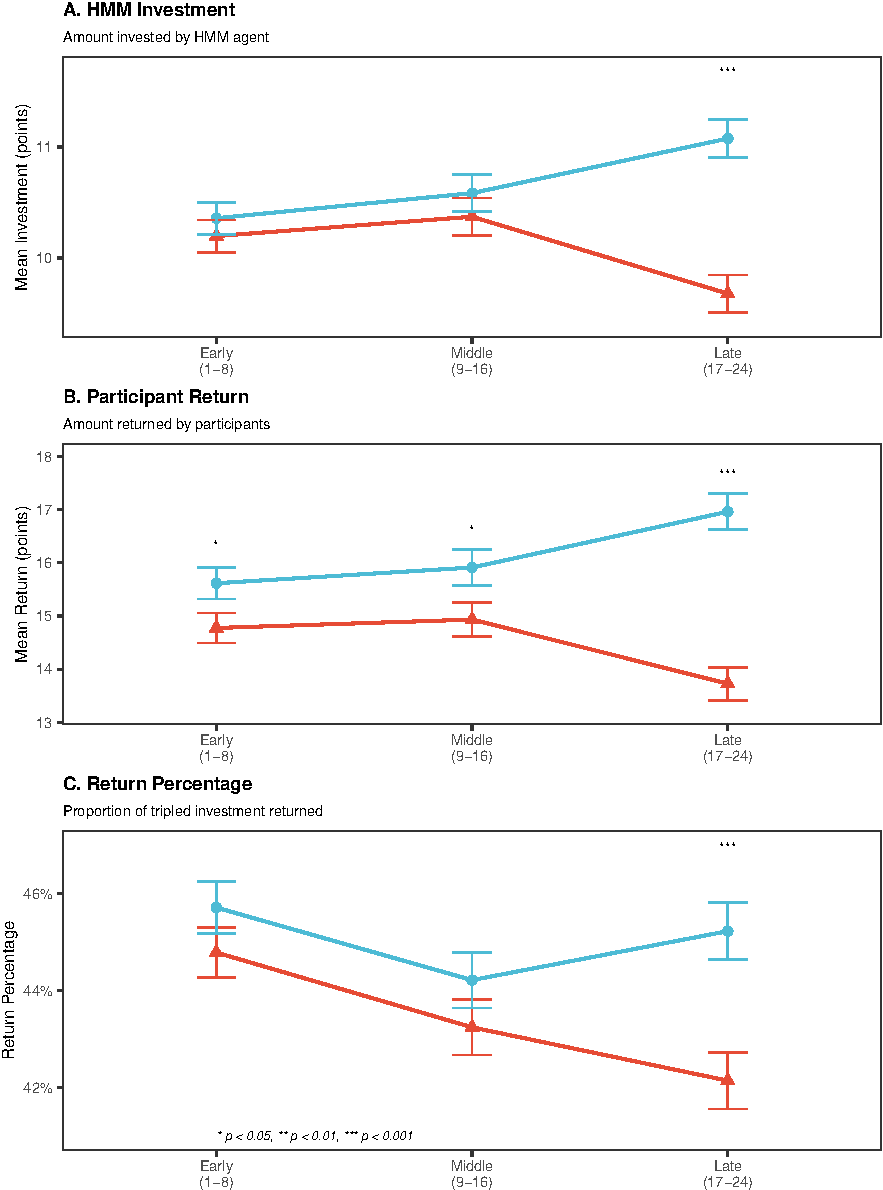
\includegraphics[width=0.9\linewidth]{article_files/figure-latex/gamesPlot2-1} \caption{Investment and return patterns across game periods by D-factor level. (A) Mean investments from HMM agents decrease for High-D participants in late game periods. (B) Absolute returns similarly decrease for High-D participants. (C) Return percentages show High-D participants consistently return a smaller proportion of received investments, with the difference becoming significant in later phases. Error bars represent standard errors of the mean. This pattern demonstrates how High-D participants' decreasing reciprocity triggers defensive responses from HMM agents.}\label{fig:gamesPlot2}
\end{figure}

\subsection{Last Round Analysis}\label{last-round-analysis}

In the last round, high\_D participants sent back significantly lower absolute returns than low\_D participants (t(358.42) = -2.31, p = 0.021); Wilcoxon W = 14504, p = 0.025). Similarly, high\_D participants sent back a significantly lower percentage of the tripled investment (t(363.98) = -2.18, p = 0.030); Wilcoxon W = 14445, p = 0.021). Both parametric (t-test) and non parametric tests (Wilcoxon) show significant differences.

\subsection{Total Payoff Analysis}\label{total-payoff-analysis}

Finally, we analyzed the total payoffs earned by participants across both games, comparing high\_D and low\_D individuals. This analysis aimed to determine whether differences in strategy observed during the game (particularly in the later periods) translated into overall differences in earnings. We used a Welch's t-test and a Wilcoxon rank-sum test.

The results showed no significant difference in total payoffs between high\_D and low\_D participants (t(180.99) = -0.17, p = 0.862; Wilcoxon W = 4253, p = 0.853).

Although high-D participants sent back lower returns in the late period of the trust game, their total accumulated payoff across all rounds was not significantly different from that of low-D participants. This seemingly paradoxical result can be explained by the adaptive behavior of the HMM opponent. While high-D individuals adopted a less cooperative strategy in later rounds, keeping a larger portion of the returns for themselves, the HMM responded by reducing its investments in these individuals. Therefore, the higher proportion kept by high-D participants was offset by a reduction in the amount they received, leading to similar overall earnings compared to the more cooperative low-D participants.

\subsection{Round by round analysis}\label{round-by-round-analysis}

To analyse participants behavior on a round by round basis, we look at the fit results from the linear mixed effects model of participant percentage returns detailed in the methods section.

\subsubsection{Main Effects}\label{main-effects}

We found a significant main effect of investment amount (\(F(1, 344.27) = 10.38\), \(p = .001\)), with participants returning higher percentages when they received larger investments, demonstrating positive reciprocity. We also found a significant main effect of round number (\(F(1, 8147.38) = 21.47\), \(p < .001\)), showing that return percentages generally decreased over time as the game progressed.

\subsubsection{D-Factor by Round Number Interaction}\label{d-factor-by-round-number-interaction}

We found a significant interaction between D-factor and round number (\(F(1, 8147.38) = 6.91\), \(p = .009\)). Participants with High-D scores demonstrated a significant negative slope in their return proportions as the game progressed, indicating a systematic decrease in reciprocity over time (slope = -0.0016, 95\% CI {[}-0.0023, -0.0010{]}). In contrast, participants with Low-D scores maintained relatively stable return rates across rounds, with a slope not significantly different from zero. The difference between these slopes was statistically significant (z = -2.64, p = 0.008).

\subsubsection{D-Factor, Opponent Type and Investment Interaction}\label{d-factor-opponent-type-and-investment-interaction}

Low-D participants showed significant positive reciprocity with both opponents: a one-unit increase in investment led to a significant increase in return percentage for both the human-like HMM (2.1\%, \emph{p} = 0.011) and the responsive HMM (3.1\%, \emph{p} = 0.000).

In contrast, High-D participants did \emph{not} show significant reciprocity with either the human-like HMM (slope = 0.008, \emph{p} = 0.314) or the responsive HMM (slope = 0.005, \emph{p} = 0.509), indicating their returns were less influenced by investment amount.

\subsubsection{Four-Way Interaction: Opponent, Investment, D-factor, and Round Number}\label{four-way-interaction-opponent-investment-d-factor-and-round-number}

\begin{figure}

{\centering 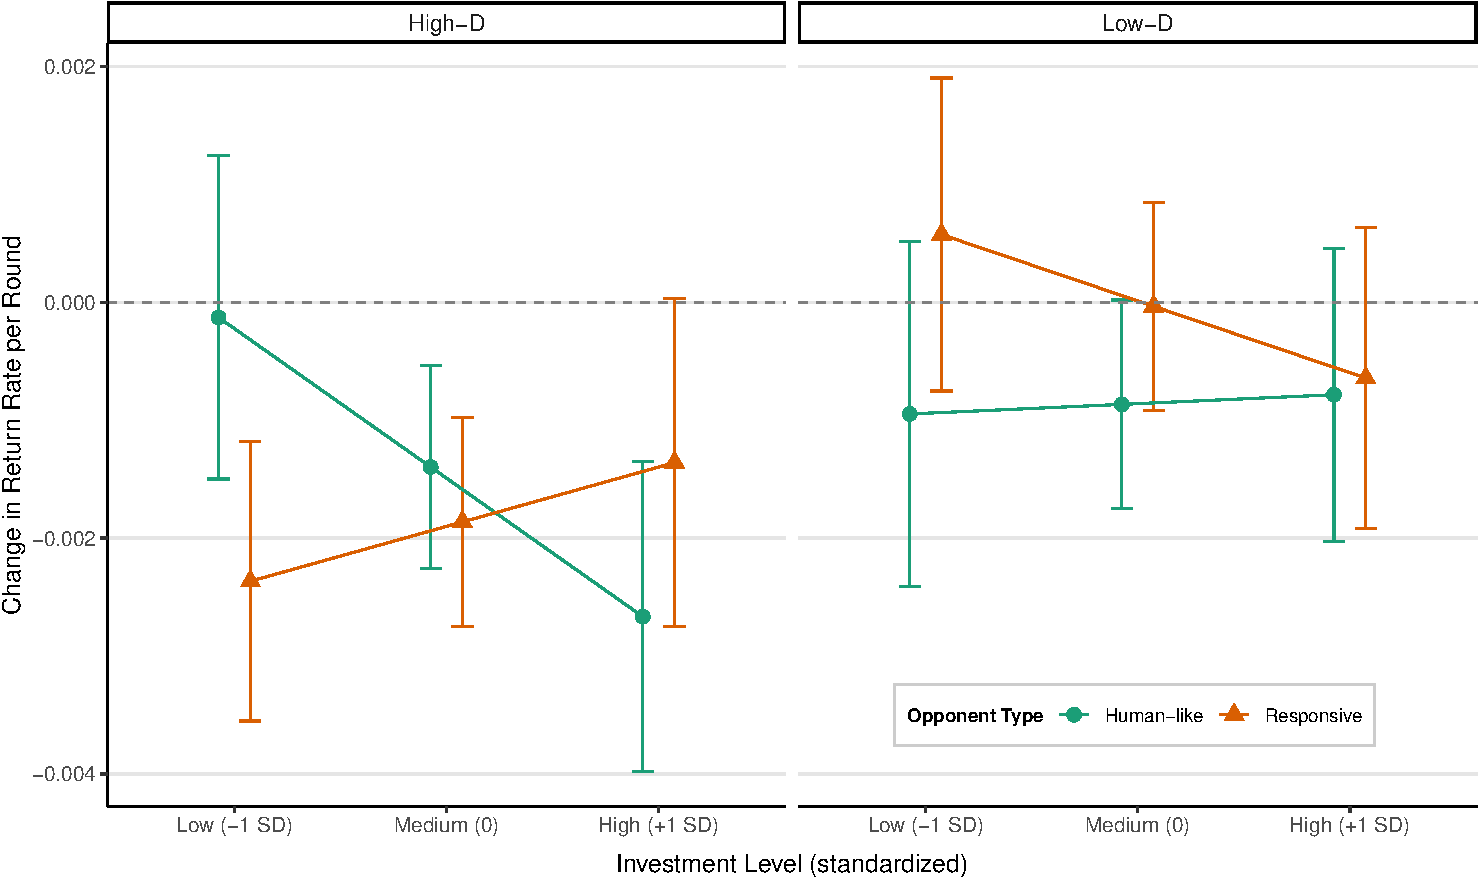
\includegraphics{article_files/figure-latex/oppExploit-1} 

}

\caption{Changes in return rate over successive rounds by investment level, opponent type, and D-factor group. Bars represent the estimated slope coefficients (change in return percentage per round) with error bars showing 95 percent confidence intervals. Negative values indicate decreasing reciprocity over time. High-D participants show more pronounced decreases in return rates, particularly with the human-like opponent at high investment levels, suggesting they learned strategic exploitation of predictable, trusting partners}\label{fig:oppExploit}
\end{figure}

Analysis of the significant four-way interaction (\(F(1, 8215.95) = 5.92\), \(p = .015\)), visualised in Figure \ref{fig:oppExploit}, revealed that only High-D participants facing the human-like opponent showed investment-dependent changes in behavior across rounds (p = 0.042). For these participants, returns decreased significantly across rounds with high investments (slope = -0.00267, 95\% CI {[}-0.00398, -0.00135{]}), but remained stable with low investments (slope = -0.00013, 95\% CI {[}-0.00150, 0.00124{]}), a significant difference in slopes (p = 0.042).

Neither Low-D participants nor High-D participants facing the responsive opponent showed this strategic pattern. This suggests High-D participants specifically exploit a weakness in Human-like opponent strategies (the propensity to remain in a mid-trust state even after receiving lower returns) by systematically reducing reciprocity over time on the most lucrative (high-investment) trials.

\begin{figure}[H]

{\centering 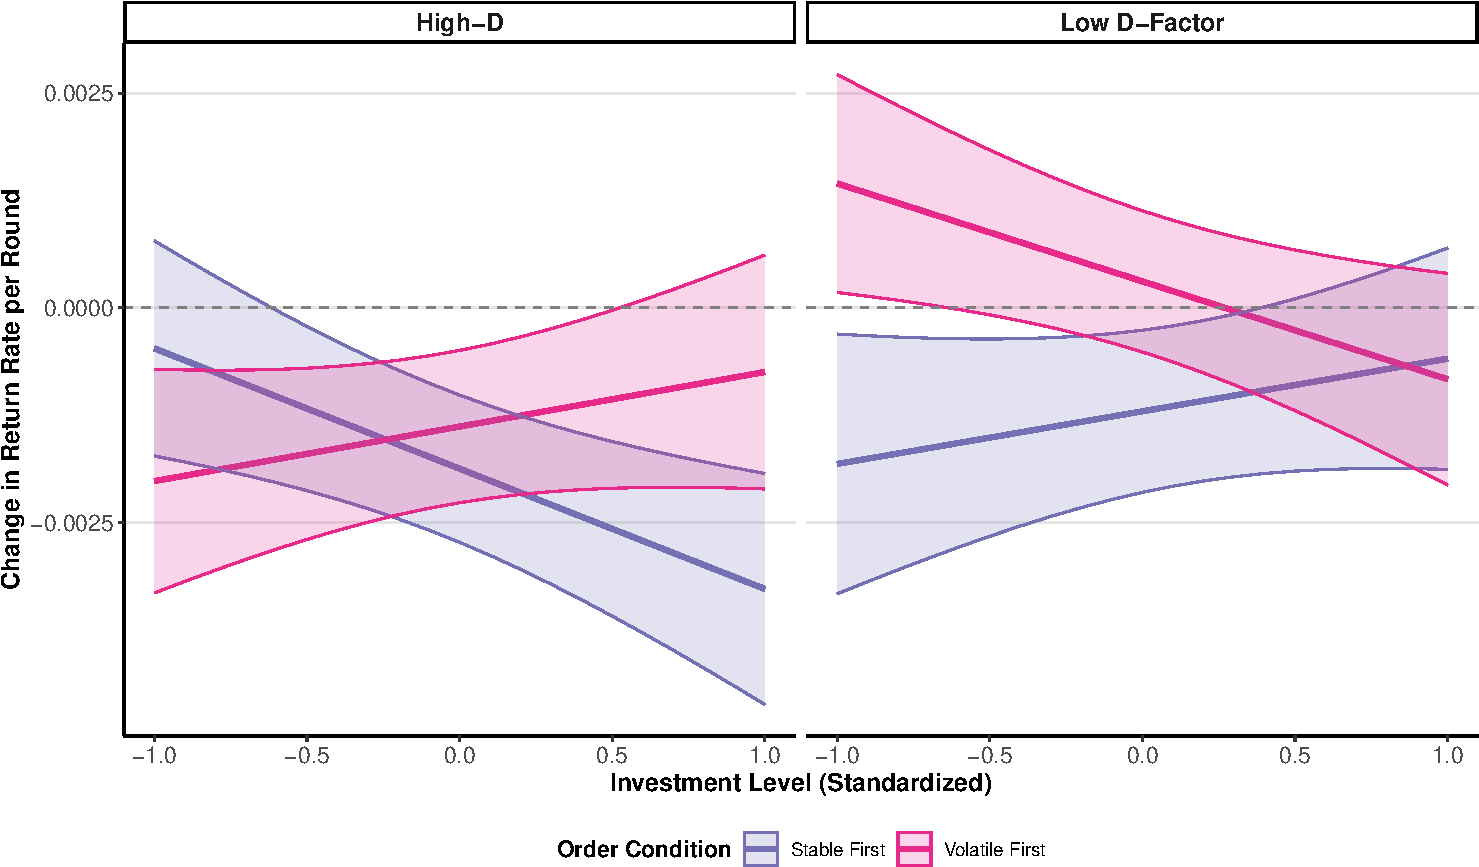
\includegraphics{article_files/figure-latex/orderEffectPlot-1} 

}

\caption{Effect of game order on changes in return rate across rounds at different investment levels. Lines represent the estimated slope coefficients (change in return rate per round) with shaded areas showing 95 percent confidence intervals. Negative values indicate decreasing reciprocity over time. High-D participants who played against the stable opponent first showed strategic exploitation primarily at high investment levels, while those who faced the volatile opponent first showed different strategic patterns. Low D-factor participants maintained more consistent return rates regardless of order condition.}\label{fig:orderEffectPlot}
\end{figure}

\subsubsection{Four-Way Interaction: Investment, Order, D-factor, and Round Number}\label{four-way-interaction-investment-order-d-factor-and-round-number}

The significant four-way interaction involving investment amount, order of opponent presentation (responsive first or stable/human-like first), D-factor, and round number (\(F(1, 8209.77) = 14.07\), \(p < .001\)) reveals a complex interplay of factors influencing return behavior. As seen in Figure \ref{fig:orderEffectPlot}, The key finding is that the \emph{order} in which participants faced the opponents, combined with their D-factor level, influenced how their returns changed over time \emph{depending on the investment level}.

High-D participants who faced the \emph{stable} (human-like) \emph{opponent} \emph{first} showed a strategic pattern: they significantly decreased their returns over rounds for \emph{high} (slope = -0.00328, p \textless{} .001) and \emph{medium} investments (slope = -0.00188, p \textless{} .001), but not for low investments (slope = -0.00047, p = 0.841). This reinforces the idea that high-D individuals are more likely to reduce cooperation when they perceive an opportunity for greater gain (higher investments) and a predictable partner. In contrast, high-D participants who faced the \emph{responsive} \emph{opponent} \emph{first} showed the \emph{opposite} pattern: decreasing returns for \emph{low} (slope = -0.00202, p = 0.007) and \emph{medium} investments (slope = -0.00138, p = 0.007), but not for high investments (slope = -0.00075, p = 0.629).

Low-D participants, regardless of the order in which they faced the opponents, did \emph{not} show significant changes in their returns across rounds for any investment level.

\subsection{Analysis of opponent ratings}\label{analysis-of-opponent-ratings}

Beyond behavioral measures, we also analyzed participants' explicit evaluations of their opponents using linear mixed-effects models. These models assessed ratings of cooperativeness, willingness to play again, and trust based on participants' D-level, the opponent type faced, and the order of games (see Figure \ref{fig:plotRatings} for a summary).

\subsubsection{Cooperative Ratings}\label{cooperative-ratings}

Linear mixed-effects analysis revealed a significant main effect of D-level (\(F(1, 179) = 7.35\), \(p = .007\)), with Low-D participants rating their opponents as more cooperative than High-D participants (\(t(179) = -2.71\), \(p = .007\)). A significant main effect of game order (\(F(1, 179) = 10.67\), \(p = .001\)) indicated participants rated opponents in their first game as more cooperative than those in their second game (\(t(179) = 3.27\), \(p = .001\)). Additionally, there was a significant main effect of opponent type (\(F(1, 179) = 5.31\), \(p = .022\)), with Human-like HMM opponents receiving higher cooperative ratings than Responsive opponents (\(t(179) = 2.31\), \(p = .022\)).

\subsubsection{Play Again Ratings}\label{play-again-ratings}

Analysis of participants' willingness to play with the same opponent again revealed a significant main effect of game order (\(F(1, 179) = 13.83\), \(p < .001\)), with participants generally more willing to play again with opponents from their first game (\(t(179) = 3.72\), \(p < .001\)). This main effect was qualified by a significant D-level × Game Order interaction (\(F(1, 179) = 4.05\), \(p = .046\)). Post-hoc analyses revealed that in the first game, High-D participants were significantly less willing to play again with their opponents compared to Low-D participants (\(t(320.47) = -2.37\), \(p = .018\)), while no such difference existed in the second game (\(t(320.47) = -0.07\), \(p = .947\)). Examining changes across games, Low-D participants showed a significant decrease in willingness to play again from the first to the second game (\(t(179) = 4.05\), \(p < .001\)), while High-D participants maintained consistent ratings across games (\(t(179) = 1.21\), \(p = .229\)).

\subsubsection{Trusting Ratings}\label{trusting-ratings}

For trust ratings, significant main effects were observed for D-level (\(F(1, 179) = 7.53\), \(p = .007\)), game order (\(F(1, 179) = 7.21\), \(p = .008\)), and opponent type (\(F(1, 179) = 4.62\), \(p = .033\)). These effects were qualified by a significant three-way interaction between D-level, game order, and opponent type (\(F(1, 179) = 4.76\), \(p = .030\)).

Post-hoc analyses revealed a complex pattern of trust perceptions. High-D participants rated Human-like opponents as significantly less trusting than Low-D participants in the first game (\(t(314.81) = -2.96\), \(p = .003\)). In contrast, High-D participants rated Responsive opponents as significantly less trusting than Low-D participants in the second game (\(t(314.81) = -2.70\), \(p = .007\)). Low-D participants showed a significant \emph{increase} in trust ratings for Human-like opponents from the first to the second game (\(t(314.81) = 2.22\), \(p = .027\)), while High-D participants showed a significant \emph{decrease} in trust ratings for Responsive opponents from the first to the second game (\(t(314.81) = 2.47\), \(p = .014\)). Additionally, High-D participants in the second game differentiated between opponent types, rating Human-like opponents as significantly more trusting than Responsive opponents (\(t(314.81) = 2.51\), \(p = .013\)).

In summary, participants with higher Dark Factor scores demonstrated consistently more negative perceptions of their opponents, particularly regarding cooperation and trust. The pattern of results indicates that individual differences in Dark Factor traits influence not only the overall level of opponent ratings but also how these ratings change across repeated interactions and between different opponent types. Notably, Low-D participants showed greater sensitivity to game order, with more pronounced decreases in ratings from first to second game, while High-D participants demonstrated greater discrimination between opponent types in their trust ratings.

\begin{figure}[H]

{\centering 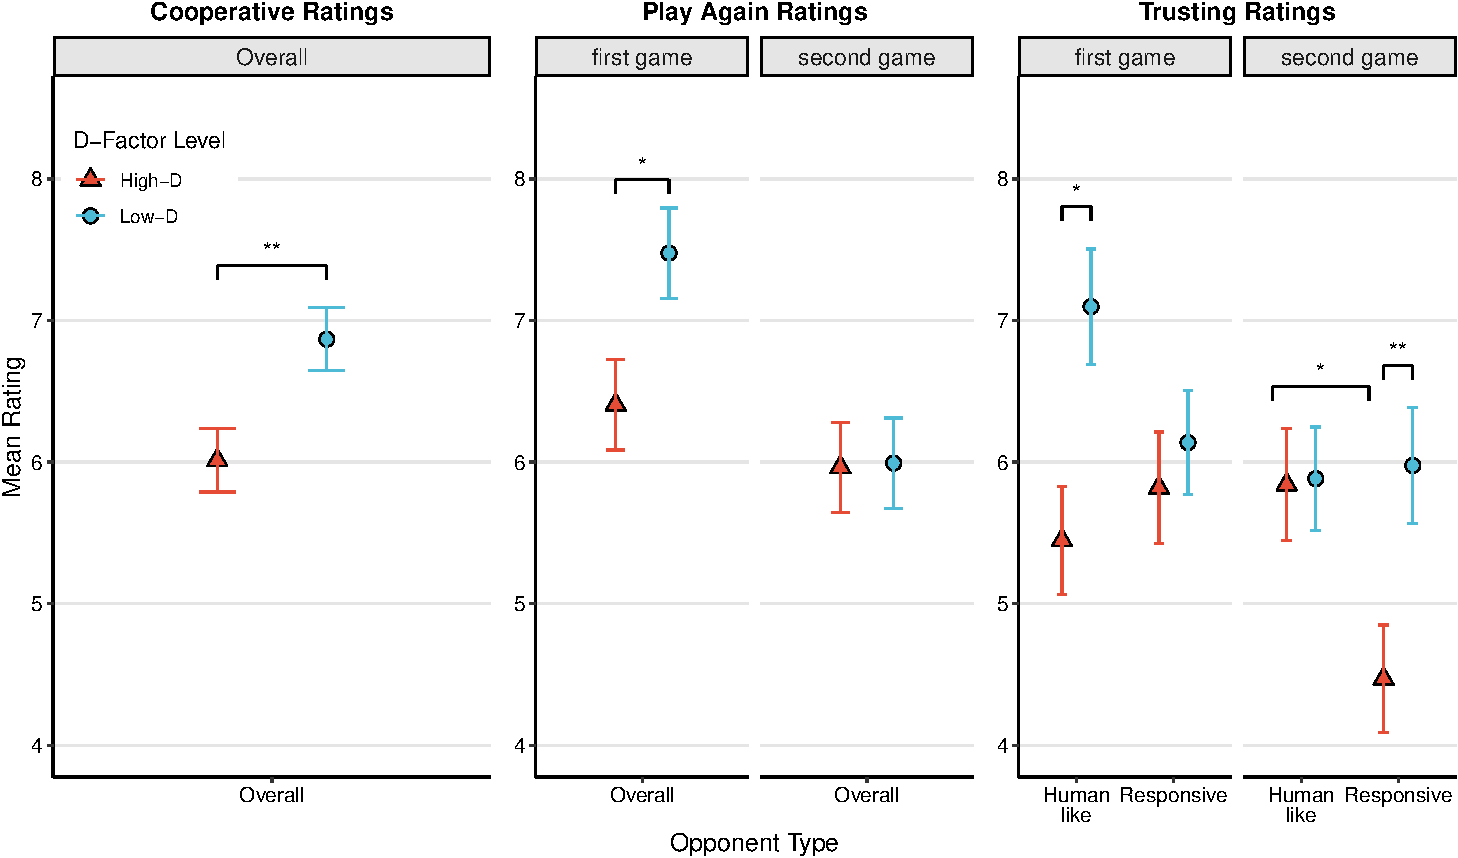
\includegraphics{article_files/figure-latex/plotRatings-1} 

}

\caption{Averages and standard errors of the participants ratings of the opponent (y-axis) by each game and d-factor group for each opponent (x-axis). The left panel represents participants' perception of co-player cooperativeness, the right one one indicates perceived co-player trust rating, and the middle panel shows the participants' willingness to play again with the same co-player. Cooperation, trust perception, and willingness to play again ratings were generally lower for the high DFP group}\label{fig:plotRatings}
\end{figure}

\subsection{Debrief questions}\label{debrief-questions}

Around 57\% of participants either thought that they played against a human opponent or were not sure whether the investor was a human or a machine.

\section{Computational Modelling}\label{computational-modelling}

TBC

\section{Discussion}\label{discussion}

The present study investigated how the Dark Factor of Personality (D-factor) influences behavior in repeated trust games, focusing on trustworthiness patterns, strategic adaptation, and perception of counterparts. Our findings reveal nuanced relationships between dark personality traits and economic decision-making that both confirm and challenge existing theoretical frameworks.

Our results demonstrated significant behavioral differences between individuals with high and Low-D scores. High-D participants consistently returned lower proportions of investment compared to their Low-D counterparts, with this difference becoming particularly pronounced in later rounds of the game. This pattern aligns with the fundamental definition of the D-factor as ``the general tendency to maximize one's utility at the expense of others, accompanied by beliefs that serve as justifications'' (Moshagen, Hilbig, and Zettler 2018). The lower return percentages directly translate to greater self-benefit at the investor's expense, supporting the construct validity of the D-factor in predicting economic behavior.
Interestingly, the timing of these differences suggests a strategic component to this behavior. The absence of significant differences in early rounds, followed by emerging disparities in later stages of interaction, indicates a possible exploitation pattern that develops over time. This temporal dimension of trustworthiness aligns with prior research suggesting that dark personality traits may manifest most strongly after establishing a baseline relationship (Jones and Paulhus 2009). This finding extends previous work on dark traits in one-shot economic games (Zhao and Smillie 2015; Thielmann and Hilbig 2019) by demonstrating how these tendencies unfold over repeated interactions.

The significant interaction between D-factor, investment amount, round number, and opponent type reveals sophisticated strategic differences between high and Low-D individuals. When facing the predictable human-like HMM opponent, High-D participants demonstrated a distinct pattern: they significantly decreased their returns over time for high-investment trials while maintaining relatively stable returns for low-investment trials. This selective exploitation strategy suggests a calculated approach to maximize gains while minimizing the risk of triggering retaliation from the investor.
This pattern is particularly significant because it represents a form of Machiavellian exploitation that targets situations of high trust (indicated by higher investments) rather than indiscriminate exploitation across all conditions. By selectively reducing reciprocity in high-stake interactions, High-D individuals effectively exploit the trust placed in them when the potential gains are greatest. This finding aligns with the conceptualization of Machiavellianism as involving strategic, long-term orientation to personal gain (Jones and Paulhus 2009) and supports previous research indicating that dark personality traits are associated with strategic rather than impulsive exploitation (Gunnthorsdottir, McCabe, and Smith 2002).
Notably, this strategic exploitation pattern was only observed with the more predictable human-like HMM opponent, not with the Responsive opponent. This distinction suggests that High-D individuals may be particularly adept at identifying and exploiting predictable social dynamics, while showing more caution in Responsive or unpredictable social environments. This contextual sensitivity adds important nuance to our understanding of how dark personality traits manifest in economic decisions.

The significant four-way interaction involving investment, order of opponent presentation, D-factor, and round number further illuminates the adaptive nature of exploitation strategies. High-D participants who first encountered the stable (human-like) opponent showed decreasing returns over rounds for high and medium investments but maintained stable returns for low investments. In contrast, those who initially faced the Responsive opponent reduced returns for low and medium investments while maintaining returns for high investments.
This pattern suggests that High-D individuals rapidly adapt their exploitation strategies based on initial experiences. When first exposed to a predictable environment, they learn to exploit high-trust situations. Conversely, when first exposed to volatility, they adopt a more conservative strategy that maintains cooperation in high-stake interactions while reducing reciprocity in lower-risk situations. This adaptive learning demonstrates sophisticated social intelligence that may underlie the effectiveness of dark personality traits in navigating complex social environments.
Low-D participants, regardless of the order in which they faced opponents, maintained relatively stable return rates across rounds and investment levels, suggesting a more consistent approach to reciprocity that is less influenced by strategic considerations or learning effects. This stability in cooperative behavior may reflect stronger adherence to fairness norms and less susceptibility to exploitative tendencies.

The analysis of opponent ratings revealed that D-factor scores significantly influenced how participants perceived their counterparts. High-D participants consistently rated their opponents lower on cooperativeness, trustworthiness, and desirability for future interaction, regardless of the opponent's actual behavior. This negative perceptual bias is consistent with research suggesting that individuals with dark personality traits may have distorted social perceptions that justify exploitation (Moshagen, Hilbig, and Zettler 2018; Zettler, Moshagen, and Hilbig 2021).
The interaction between D-factor, game order, and opponent type for trust ratings suggests complex differences in how high and Low-D individuals update their social perceptions based on experience. While Low-D participants showed increased trust in human-like opponents from first to second game, High-D participants showed decreased trust in Responsive opponents. This differential updating may reflect differences in attribution processes: Low-D individuals may attribute positive interactions to stable traits of their partner, while High-D individuals may be more sensitive to negative interactions and use them to justify subsequent exploitation.
These findings extend beyond economic behavior to suggest that the D-factor influences the entire process of social perception and decision-making. The negative bias in opponent evaluation may serve as a cognitive mechanism that facilitates exploitation by reducing empathic concern and moral constraints associated with harming a positively regarded other.

The analysis of final-round behavior, where participants knew there would be no further interactions, provides insight into purely self-interested tendencies without the strategic considerations of reputation building. In these last rounds, High-D participants returned significantly lower amounts than Low-D participants, both in absolute terms and as a percentage of investment. This finding represents a clear manifestation of the maximizing self-interest component of the D-factor when strategic constraints are removed.
The last-round effect essentially transforms the trust game into a dictator game, where participants can freely decide how much to return without fear of future consequences. The significant D-factor difference in this context aligns with previous research showing associations between the D-factor and selfish behavior in dictator games (Moshagen, Hilbig, and Zettler 2020). The consistency across economic paradigms strengthens the conclusion that the D-factor represents a stable tendency toward self-maximization when social constraints are minimal.

A particularly interesting finding was that despite returning lower percentages, High-D participants did not achieve significantly higher total payoffs compared to Low-D participants. This seemingly paradoxical result can be explained by the adaptive nature of the HMM opponent, which reduced investments in response to lower returns from High-D participants. This dynamic illustrates how exploitative strategies may fail to maximize long-term gains in environments with responsive counterparts, as initial exploitation triggers defensive reactions that ultimately limit future opportunities for gain.
This outcome has important implications for understanding the evolutionary stability of dark personality traits. While the D-factor may confer advantages in certain one-shot interactions or where reputation effects are minimal, its effectiveness as a long-term strategy in repeated interactions with responsive partners appears limited. This aligns with theoretical accounts suggesting that dark personality traits may represent frequency-dependent strategies that are most beneficial when rare in a population (Mealey 1995), as widespread exploitation would trigger universal defensive responses that limit its effectiveness.

\subsection{Theoretical and practical implications}\label{theoretical-and-practical-implications}

Our findings have several important implications for personality psychology and behavioral economics. First, they demonstrate that the D-factor, as a unifying construct of dark personality traits, provides meaningful predictive power for understanding trustworthiness in economic exchanges. The convergent patterns of exploitation, negative social perception, and self-maximization across different measures support the conceptual coherence of the D-factor construct.
Second, our results highlight the importance of considering the temporal dimension of trust and reciprocity. The emerging differences between high and Low-D participants over repeated interactions suggest that single-round economic games may underestimate the influence of personality traits on economic behavior. Future research should continue to examine how personality influences behavioral trajectories rather than just static decision points.
Third, the interaction between D-factor and opponent volatility provides insight into the contextual sensitivity of dark personality traits. The finding that High-D individuals modulate their exploitation strategies based on opponent predictability suggests sophisticated social intelligence rather than rigid antisocial tendencies. This nuance is important for developing more accurate models of how personality influences social decision-making across different environments.
Finally, our findings have practical implications for promoting cooperation in economic exchanges. The fact that High-D participants received lower investments over time indicates that exploitative strategies trigger defensive responses that ultimately limit opportunities for mutual gain. Interventions that highlight these long-term consequences might help redirect self-interested motivations toward more sustainable cooperative strategies.

\subsection{Limitations and future directions}\label{limitations-and-future-directions}

Several limitations of the current study suggest directions for future research. First, while we observed clear behavioral differences between high and Low-D individuals, our design cannot determine which specific aspects of the D-factor (e.g., Machiavellianism, psychopathy, or narcissism) drive these effects. Future studies could include measures of these specific traits alongside the D-factor to examine their relative contributions.
Second, our use of HMM opponents provided excellent experimental control but may limit ecological validity. Future research could examine D-factor influences in fully human interactions to capture the richer social dynamics of real-world trust building.
Finally, while we found significant differences in behavior and perception, we did not explore the underlying affective or cognitive processes that mediate these effects. Future studies could incorporate measures of empathy, moral disengagement, or social value orientation to understand how dark personality traits influence the subjective experience of economic exchanges.

\section{Conclusion}\label{conclusion}

This study provides novel insights into how the Dark Factor of Personality influences behavior in repeated trust games. Our findings demonstrate that individuals with High-D scores exhibit systematic patterns of lower reciprocity that emerge most strongly in later rounds of interaction, particularly when facing predictable opponents and receiving high investments. These behavioral differences are accompanied by more negative perceptions of interaction partners, suggesting a comprehensive influence of dark personality traits on both social cognition and economic decision-making.
The sophistication of exploitation strategies---adapting to opponent type, investment level, and interaction history---indicates that dark personality traits may involve complex social intelligence rather than simple antisocial tendencies. However, the failure of these exploitative strategies to yield higher total payoffs highlights the self-limiting nature of exploitation in responsive social environments.
These findings bridge the gap between personality psychology and behavioral economics, demonstrating how stable personality traits manifest in dynamic economic exchanges. They extend previous research on dark personality traits by revealing how exploitation unfolds over time and varies across contexts. Future research should continue to explore the cognitive and affective mechanisms underlying these behavioral patterns and examine how interventions might promote cooperation even among individuals with stronger exploitative tendencies.
Understanding the relationship between the D-factor and trustworthiness has significant implications for promoting cooperative outcomes in economic and social interactions. By recognizing how dark personality traits influence trust dynamics, we can develop more effective strategies for fostering cooperation and limiting the social costs of exploitation.

\section*{References}\label{references}
\addcontentsline{toc}{section}{References}

\phantomsection\label{refs}
\begin{CSLReferences}{1}{0}
\bibitem[\citeproctext]{ref-Almaatouq2021}
Almaatouq, Abdullah, Joshua Becker, James P. Houghton, Nicolas Paton, Duncan J. Watts, and Mark E. Whiting. 2021. {``{Empirica}: A Virtual Lab for High-Throughput Macro-Level Experiments.''} \emph{Behavior Research Methods} 53 (5): 2158--71. \url{https://doi.org/10.3758/s13428-020-01535-9}.

\bibitem[\citeproctext]{ref-Berg1995}
Berg, Joyce, John Dickhaut, and Kevin McCabe. 1995. {``Trust, Reciprocity, and Social History.''} \emph{Games and Economic Behavior} 10 (1): 122--42. \url{https://doi.org/10.1006/game.1995.1027}.

\bibitem[\citeproctext]{ref-Bohnet2004}
Bohnet, Iris, and Steffen Huck. 2004. {``Repetition and Reputation: {Implications} for Trust and Trustworthiness When Institutions Change.''} \emph{American Economic Review} 94 (2): 362--66. \url{https://doi.org/10.1257/0002828041301506}.

\bibitem[\citeproctext]{ref-Camerer2003}
Camerer, Colin F. 2003. \emph{Behavioral Game Theory: {Experiments} in Strategic Interaction}. Princeton University Press.

\bibitem[\citeproctext]{ref-Charness2008}
Charness, Gary, Ramon Cobo-Reyes, and Natalia Jiménez. 2008. {``An Investment Game with Third-Party Intervention.''} \emph{Journal of Economic Behavior \& Organization} 68 (1): 18--28. \url{https://doi.org/10.1016/j.jebo.2008.02.006}.

\bibitem[\citeproctext]{ref-Fiedler2011}
Fiedler, Martin, Ernan Haruvy, and Sherry Xin Li. 2011. {``Social Distance in a Virtual World Experiment.''} \emph{Games and Economic Behavior} 72 (2): 400--426. \url{https://doi.org/10.1016/j.geb.2010.09.004}.

\bibitem[\citeproctext]{ref-Gong2019}
Gong, Xiaoxiao, Inti A. Brazil, Luke J. Chang, and Alan G. Sanfey. 2019. {``Psychopathic Traits Are Related to Diminished Guilt Aversion and Reduced Trustworthiness During Social Decision-Making.''} \emph{Scientific Reports} 9 (1): 7307. \url{https://doi.org/10.1038/s41598-019-43727-0}.

\bibitem[\citeproctext]{ref-Gunnthorsdottir2002}
Gunnthorsdottir, Anna, Kevin McCabe, and Vernon Smith. 2002. {``Using the {Machiavellianism} Instrument to Predict Trustworthiness in a Bargaining Game.''} \emph{Journal of Economic Psychology} 23 (1): 49--66. \url{https://doi.org/10.1016/S0167-4870(01)00067-8}.

\bibitem[\citeproctext]{ref-Ibanez2016}
Ibáñez, Marı́a I., Gerardo Sabater-Grande, Ivan Barreda-Tarrazona, Laura Mezquita, Sara López-Ovejero, Héctor Villa, Pandelis Perakakis, Generos Ortet, Aurora Garcı́a-Gallego, and Nikolaos Georgantzı́s. 2016. {``Take the Money and Run: {Psychopathic} Behavior in the Trust Game.''} \emph{Frontiers in Psychology} 7: 1866. \url{https://doi.org/10.3389/fpsyg.2016.01866}.

\bibitem[\citeproctext]{ref-Jones2009}
Jones, Daniel N., and Delroy L. Paulhus. 2009. {``{Machiavellianism}.''} In \emph{Handbook of Individual Differences in Social Behavior}, edited by Mark R. Leary and Rick H. Hoyle, 93--108. The Guilford Press.

\bibitem[\citeproctext]{ref-Matuschek2017}
Matuschek, Hannes, Reinhold Kliegl, Shravan Vasishth, Harald Baayen, and Douglas Bates. 2017. {``Balancing {Type I} Error and Power in Linear Mixed Models.''} \emph{Journal of Memory and Language} 94: 305--15. \url{https://doi.org/10.1016/j.jml.2017.01.001}.

\bibitem[\citeproctext]{ref-Mealey1995}
Mealey, Linda. 1995. {``The Sociobiology of Sociopathy: {An} Integrated Evolutionary Model.''} \emph{Behavioral and Brain Sciences} 18 (3): 523--41. \url{https://doi.org/10.1017/S0140525X00039595}.

\bibitem[\citeproctext]{ref-Moshagen2018}
Moshagen, Morten, Benjamin E. Hilbig, and Ingo Zettler. 2018. {``The Dark Core of Personality.''} \emph{Psychological Review} 125 (5): 656--88. \url{https://doi.org/10.1037/rev0000111}.

\bibitem[\citeproctext]{ref-Moshagen2020}
---------. 2020. {``The Dark Core of Personality and Socially Aversive Psychopathology.''} \emph{Journal of Personality} 88 (6): 1253--70. \url{https://doi.org/10.1111/jopy.12577}.

\bibitem[\citeproctext]{ref-Rosenberger2019}
Rosenberger, Lisa A., Dimitris Tsivilis, and Florian Müller. 2019. {``Fairness Norm Violations in Antisocial Offenders During Trust Games: {A} Repeated Trust Game Investigation.''} \emph{Personality and Individual Differences} 136: 113--21. \url{https://doi.org/10.1016/j.paid.2018.01.007}.

\bibitem[\citeproctext]{ref-Singmann2022}
Singmann, Henrik, Ben Bolker, Jake Westfall, Frederik Aust, Mattan S. Ben-Shachar, Søren Højsgaard, John Fox, et al. 2022. {``Afex: Analysis of Factorial Experiments.''} \url{https://CRAN.R-project.org/package=afex}.

\bibitem[\citeproctext]{ref-Thielmann2019}
Thielmann, Isabel, and Benjamin E. Hilbig. 2019. {``No Gain Without Pain: {The} Psychological Costs of Dishonesty.''} \emph{Journal of Economic Psychology} 71: 126--37. \url{https://doi.org/10.1016/j.joep.2018.06.001}.

\bibitem[\citeproctext]{ref-Zettler2021}
Zettler, Ingo, Morten Moshagen, and Benjamin E. Hilbig. 2021. {``Stability and Change: {The} {Dark Factor of Personality} Shapes Dark Traits.''} \emph{Social Psychological and Personality Science} 12 (7): 974--83. \url{https://doi.org/10.1177/1948550620953288}.

\bibitem[\citeproctext]{ref-Zhao2015}
Zhao, Kaiming, and Luke D. Smillie. 2015. {``The Role of Interpersonal Traits in Social Decision Making: {Exploring} Sources of Behavioral Heterogeneity in Economic Games.''} \emph{Personality and Social Psychology Review} 19 (3): 277--302. \url{https://doi.org/10.1177/1088868314553709}.

\end{CSLReferences}

\end{document}
